% Auto-generated by figures/src/make_captions.py (numbers from figures/src/data). Usage:
% \begin{figure*}[t]\centering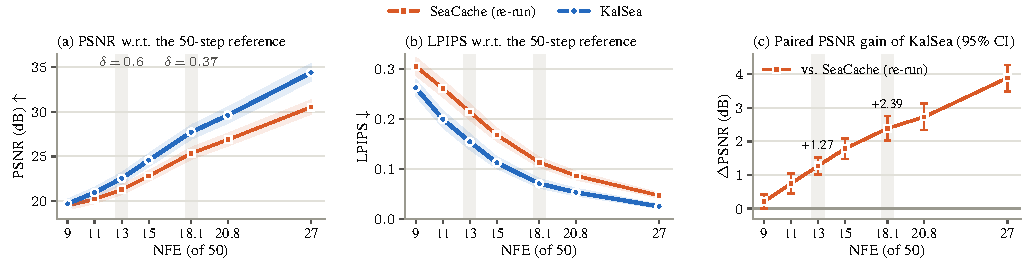
\includegraphics[width=\textwidth]{figures/fig_tradeoff.pdf}% Auto-generated by figures/src/make_captions.py (numbers from figures/src/data). Usage:
% \begin{figure*}[t]\centering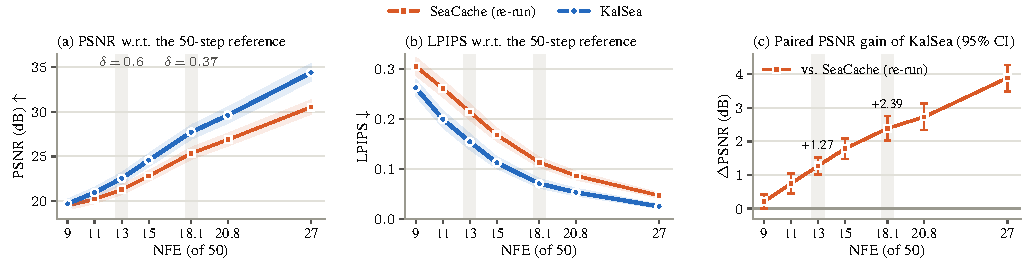
\includegraphics[width=\textwidth]{figures/fig_tradeoff.pdf}% Auto-generated by figures/src/make_captions.py (numbers from figures/src/data). Usage:
% \begin{figure*}[t]\centering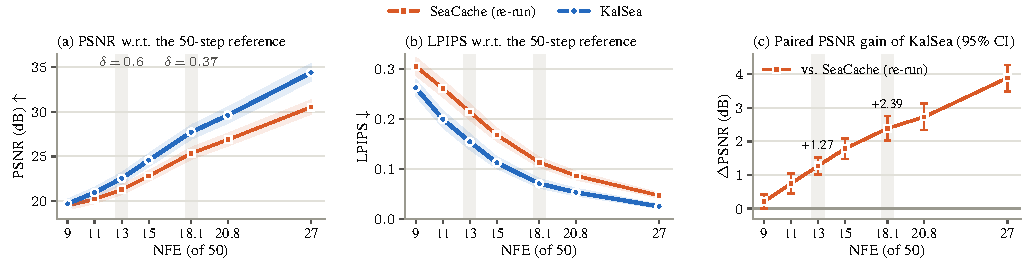
\includegraphics[width=\textwidth]{figures/fig_tradeoff.pdf}% Auto-generated by figures/src/make_captions.py (numbers from figures/src/data). Usage:
% \begin{figure*}[t]\centering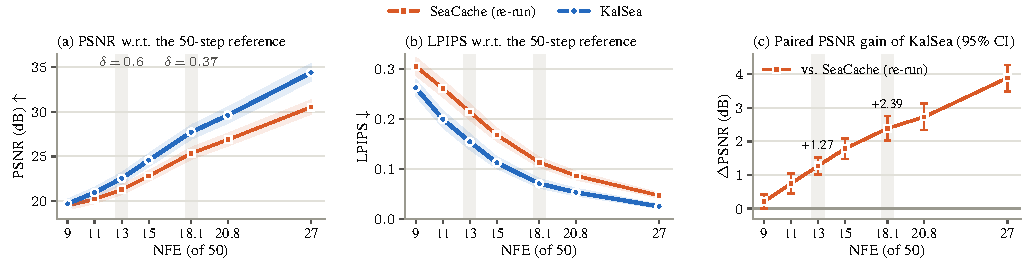
\includegraphics[width=\textwidth]{figures/fig_tradeoff.pdf}\input{figures/fig_tradeoff_caption}\end{figure*}   (one-column variant: figures/fig_tradeoff_1col.pdf, width=\columnwidth, same caption)
\caption{\textbf{Quality--compute trade-off on \flux} (DrawBench, 200 held-out prompts). \textbf{(a)}~PSNR and \textbf{(b)}~LPIPS with respect to the 50-step reference vs.\ the mean number of transformer evaluations per image (\nfe). The budget is set by the \sea-gate threshold $\delta \in \{0.2, 0.3, 0.37, 0.5, 0.6, 0.8, 1.0\}$, shared by all methods; gray bands mark the two budgets of \cref{tab:flux-main} ($\delta = 0.3$, $0.6$). Lines: means over prompts; shaded: 95\% bootstrap CIs. \textbf{(c)}~Paired per-prompt PSNR gain of \ours over \seacache and over \kalsea (mean, 95\% bootstrap CI). The gain over \seacache grows with the budget, from +0.21\,dB [$-$0.005, +0.42] at 9 \nfe (not significant; LPIPS still improves by 0.043 [0.033, 0.053]) to +3.89\,dB [+3.49, +4.28] at 27 \nfe; the gain over \kalsea (gap smoothing alone) is positive at every budget. \seacache: \sea gate with residual reuse; \kalsea: \sea gate with Kalman residual forecasting; \ours: \kalsea with predictor-corrector gap smoothing.}
\label{fig:tradeoff}
\end{figure*}   (one-column variant: figures/fig_tradeoff_1col.pdf, width=\columnwidth, same caption)
\caption{\textbf{Quality--compute trade-off on \flux} (DrawBench, 200 held-out prompts). \textbf{(a)}~PSNR and \textbf{(b)}~LPIPS with respect to the 50-step reference vs.\ the mean number of transformer evaluations per image (\nfe). The budget is set by the \sea-gate threshold $\delta \in \{0.2, 0.3, 0.37, 0.5, 0.6, 0.8, 1.0\}$, shared by all methods; gray bands mark the two budgets of \cref{tab:flux-main} ($\delta = 0.3$, $0.6$). Lines: means over prompts; shaded: 95\% bootstrap CIs. \textbf{(c)}~Paired per-prompt PSNR gain of \ours over \seacache and over \kalsea (mean, 95\% bootstrap CI). The gain over \seacache grows with the budget, from +0.21\,dB [$-$0.005, +0.42] at 9 \nfe (not significant; LPIPS still improves by 0.043 [0.033, 0.053]) to +3.89\,dB [+3.49, +4.28] at 27 \nfe; the gain over \kalsea (gap smoothing alone) is positive at every budget. \seacache: \sea gate with residual reuse; \kalsea: \sea gate with Kalman residual forecasting; \ours: \kalsea with predictor-corrector gap smoothing.}
\label{fig:tradeoff}
\end{figure*}   (one-column variant: figures/fig_tradeoff_1col.pdf, width=\columnwidth, same caption)
\caption{\textbf{Quality--compute trade-off on \flux} (DrawBench, 200 held-out prompts). \textbf{(a)}~PSNR and \textbf{(b)}~LPIPS with respect to the 50-step reference vs.\ the mean number of transformer evaluations per image (\nfe). The budget is set by the \sea-gate threshold $\delta \in \{0.2, 0.3, 0.37, 0.5, 0.6, 0.8, 1.0\}$, shared by all methods; gray bands mark the two budgets of \cref{tab:flux-main} ($\delta = 0.3$, $0.6$). Lines: means over prompts; shaded: 95\% bootstrap CIs. \textbf{(c)}~Paired per-prompt PSNR gain of \ours over \seacache and over \kalsea (mean, 95\% bootstrap CI). The gain over \seacache grows with the budget, from +0.21\,dB [$-$0.005, +0.42] at 9 \nfe (not significant; LPIPS still improves by 0.043 [0.033, 0.053]) to +3.89\,dB [+3.49, +4.28] at 27 \nfe; the gain over \kalsea (gap smoothing alone) is positive at every budget. \seacache: \sea gate with residual reuse; \kalsea: \sea gate with Kalman residual forecasting; \ours: \kalsea with predictor-corrector gap smoothing.}
\label{fig:tradeoff}
\end{figure*}   (one-column variant: figures/fig_tradeoff_1col.pdf, width=\columnwidth, same caption)
\caption{\textbf{Quality--compute trade-off on \flux} (DrawBench, 200 held-out prompts). \textbf{(a)}~PSNR and \textbf{(b)}~LPIPS with respect to the 50-step reference vs.\ the mean number of transformer evaluations per image (\nfe). The budget is set by the \sea-gate threshold $\delta \in \{0.2, 0.3, 0.37, 0.5, 0.6, 0.8, 1.0\}$, shared by all methods; gray bands mark the two budgets of \cref{tab:flux-main} ($\delta = 0.3$, $0.6$). Lines: means over prompts; shaded: 95\% bootstrap CIs. \textbf{(c)}~Paired per-prompt PSNR gain of \ours over \seacache and over \kalsea (mean, 95\% bootstrap CI). The gain over \seacache grows with the budget, from +0.21\,dB [$-$0.005, +0.42] at 9 \nfe (not significant; LPIPS still improves by 0.043 [0.033, 0.053]) to +3.89\,dB [+3.49, +4.28] at 27 \nfe; the gain over \kalsea (gap smoothing alone) is positive at every budget. \seacache: \sea gate with residual reuse; \kalsea: \sea gate with Kalman residual forecasting; \ours: \kalsea with predictor-corrector gap smoothing.}
\label{fig:tradeoff}
